\subsection{Anforderungsspezifikation}

\subsubsection{Funktionale Anforderungen}
\begin{figure}
	\centering
	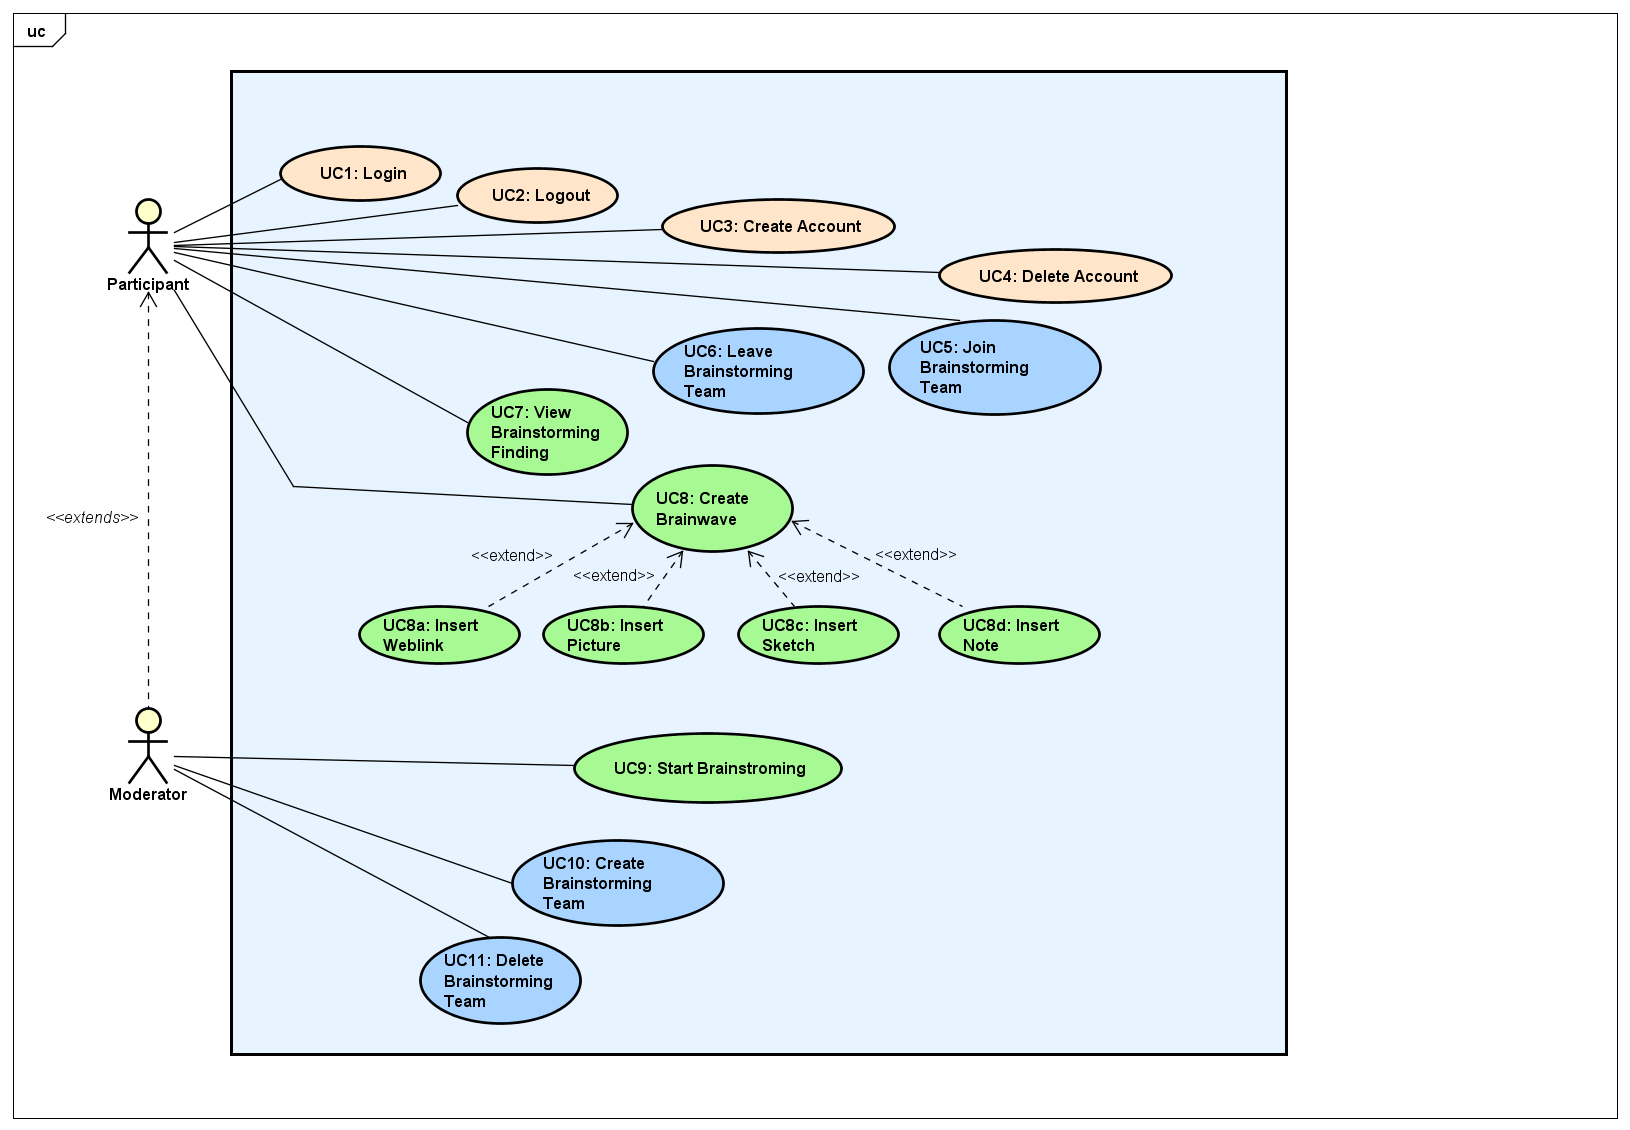
\includegraphics[width=0.7\linewidth]{./img/anforderungen/UC-Methode635.png}
	\caption{Use-Case Diagramm Methode 635}
	\label{fig:uc-methode635}
\end{figure}
%TODO: Hellfarbene UC erklären dass neu, schwachfarbene erklären, UC12 sagen dass mapping pro team 1 finding nicht mehr gültig ist, leave team unnötig, neue insert ideas (Pattern, Video)
\paragraph{Brief Use-Cases}


\paragraph{Fully-Dressed Use-Cases}


\paragraph{Abuse-Cases}
\paragraph{Sequenzdiagramm}

\subsubsection{Nicht-Funktionale Anforderungen}
Wie schon in unserer Studienarbeit halten wir uns auch hier wieder an die Standards ISO 9126\cite{ISO9126} bzw. dessen Nachfolger ISO 25010\cite{ISO9126_ISO25010}. Beide ISO-Normen sind sich sehr ähnlich und liefern eine gute Checkliste für jegliche Art von Systemanforderungen.

\begin{figure}[h]
	\centering
	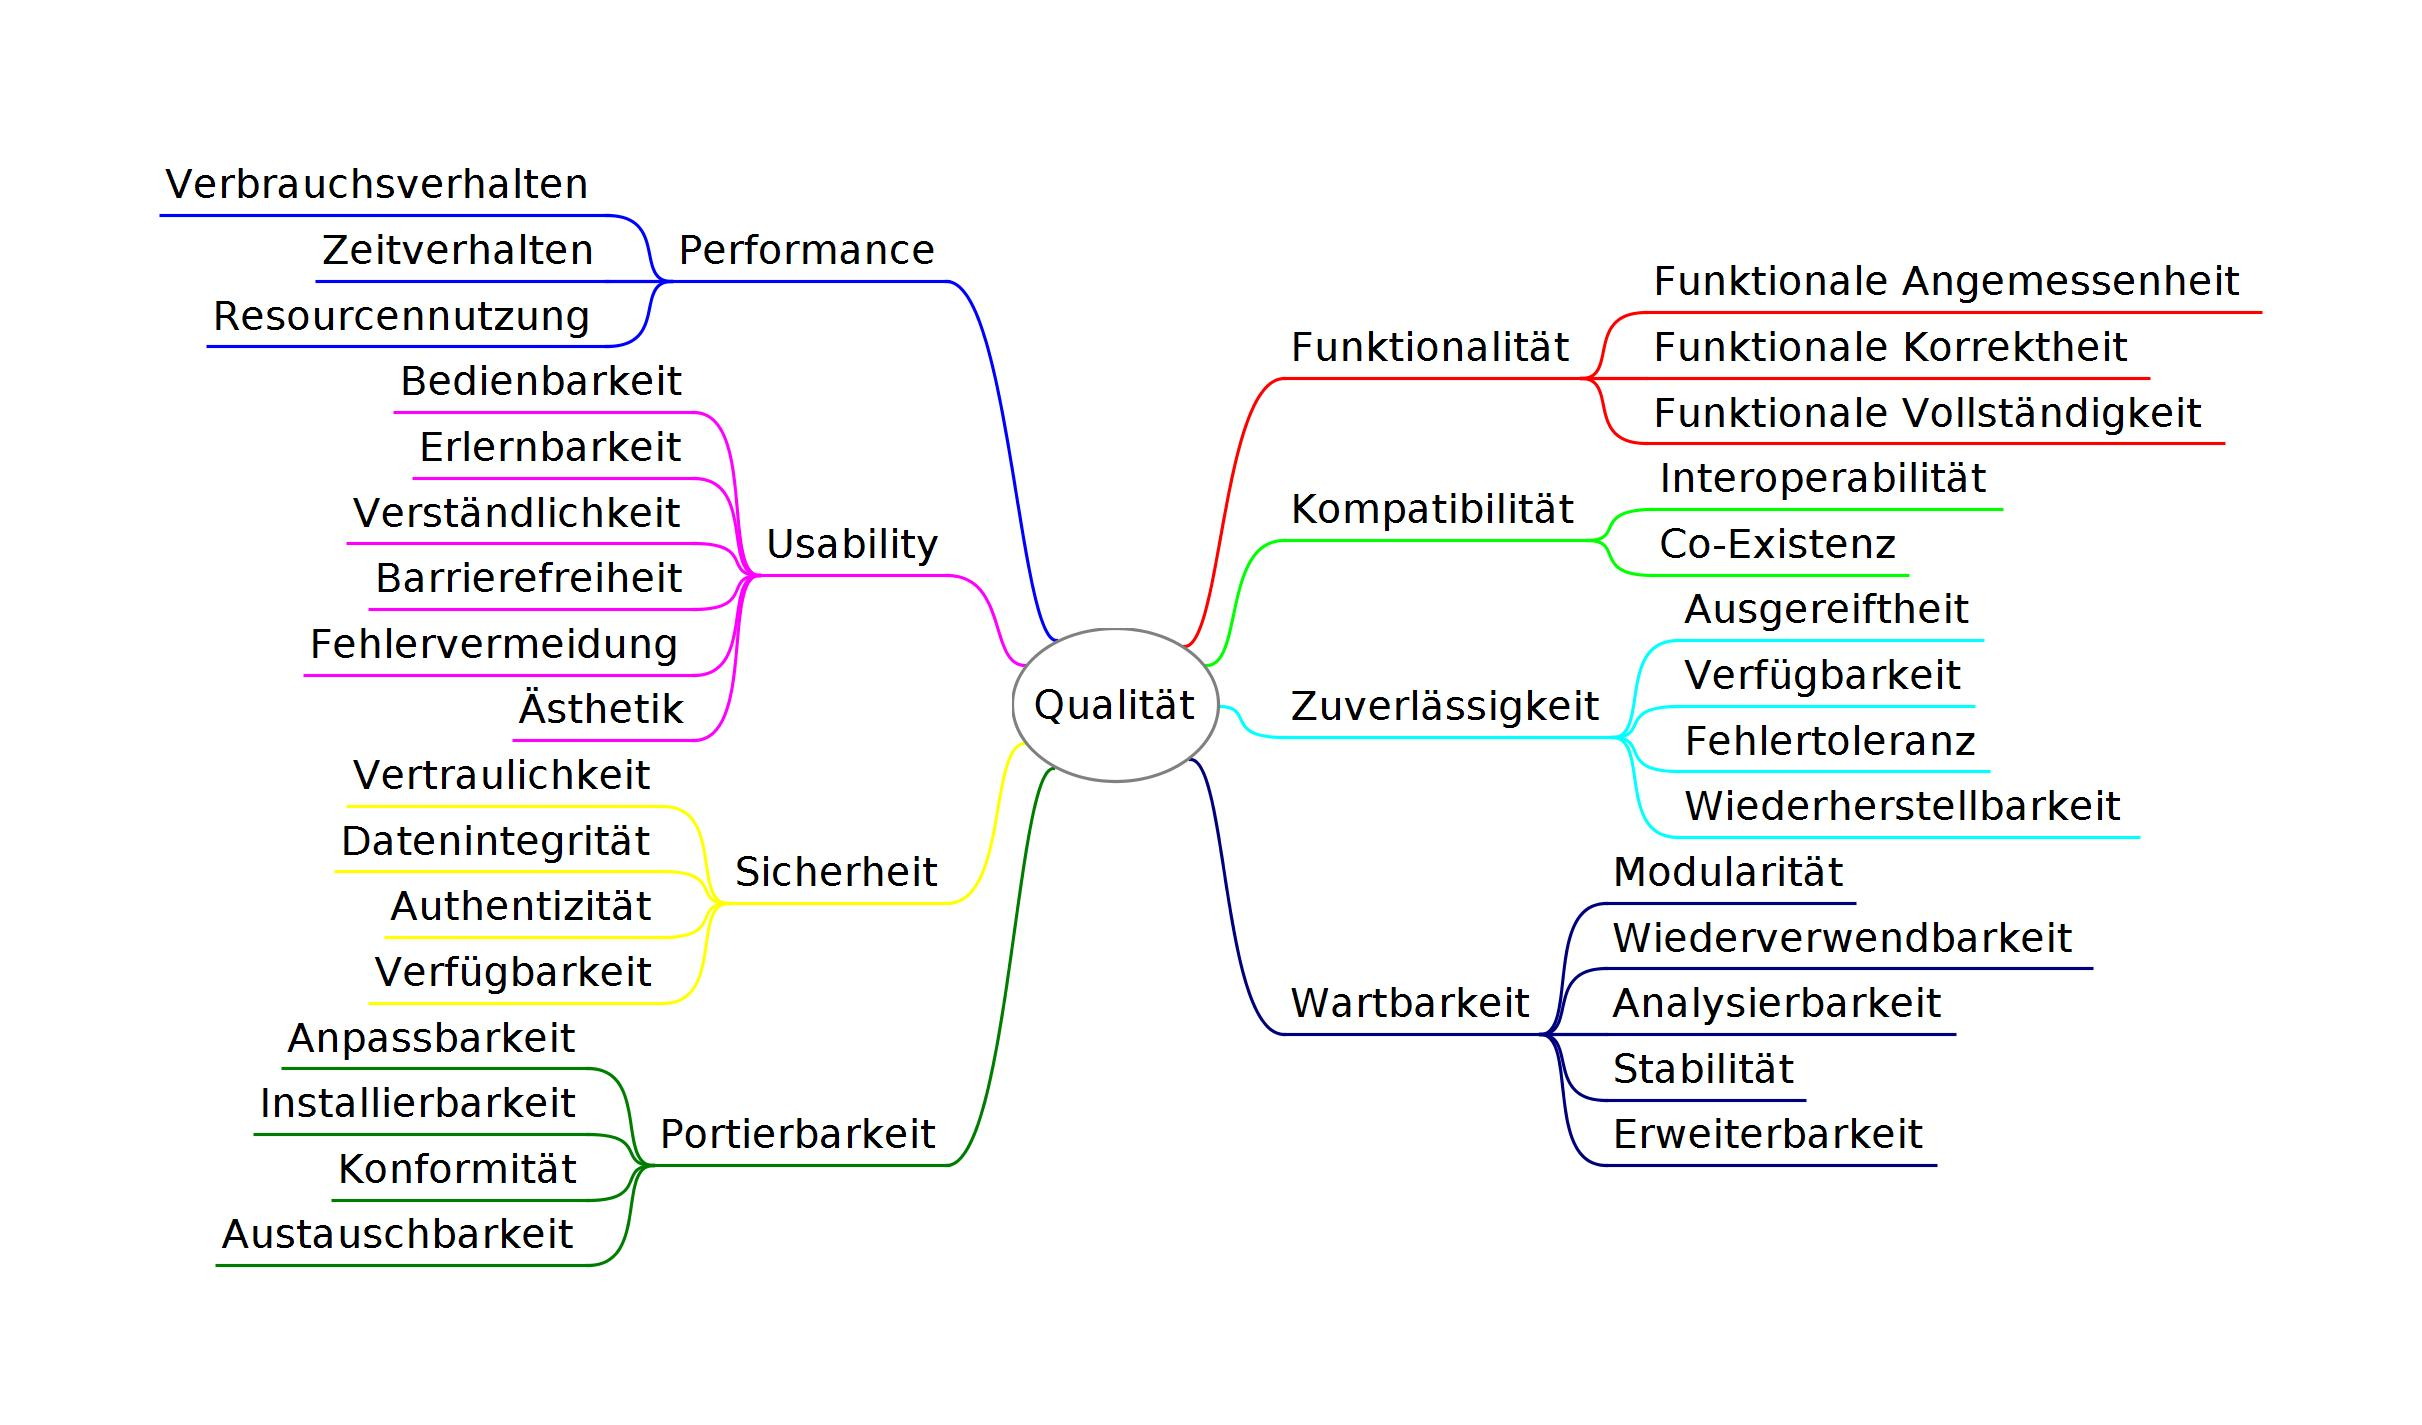
\includegraphics[width=1\linewidth]{img/anforderungen/quality}
	\caption[Anforderungskategorien nach ISO 25010]{Anforderungskategorien nach  ISO 25010}\cite{ISO25010_Bild}
	\label{fig:ISO 25010}
\end{figure}

Im Gegensatz zur Studienarbeit wollen wir uns bei dieser Arbeit aber vor allem auf Faktoren wie Erweiterbarkeit und Modularität konzentrieren. Auch sollen Faktoren wie Zeitverhalten und Ästhetik stärker in den Vordergrund rücken. 

Die bekannten nicht-funktionale Anforderungen aus der Studienarbeit bleiben allerdings weiter bestehen. Um genaue und erfüllbare nicht-funktionale Anforderungen zu definieren, müssen die SMART-Kriterien \cite{SMART} erfüllt sein.

\begin{center}
    \begin{tabular}{ | p{6cm} | p{2.5cm} | p{2.5cm} | p{2.5cm} |}
    	\hline
    Kriterium & Minimum & Optimal & Übertroffen \\ 
    	\hline
    \textbf{Zeitverhalten} \newline Zeitkritische Kommunikation (Abgabe von Ideen/Brainsheets) zwischen Server und App beträgt: & 2 Sekunden & 1 Sekunden & weniger als 1 Sekunde \\
    	\hline
    \textbf{Erweiterbarkeit} \newline Die Anzahl an neuen Modularten (Problem-Arten), welche mit der bestehenden Architektur als umsetzbar gelten, wird als ... angesehen: & zu wenig & ausreichend & unbegrenzt \\
    	\hline
    \textbf{Modularität} \newline Die App ist innert ... Tagen um ein neues Modul (Problem-Art) erweitert: & 5 Tage & 2 Tage & weniger als 1 Tag \\
    	\hline
    \textbf{Ästhetik} \newline Die Anziehungskraft gegenüber dem Endnutzer wird als ... charakterisiert: & gering & in Ordnung & süchtig \\
    	\hline
    \textbf{Ausgereiftheit} \newline Der Grad der Ausgereiftheit oder Reife wird als ... angesehen: & ungenügend für den produktiven Einsatz (Prototypen-Stadium) & genügend für den produktiven Einsatz, kann aber immer noch in Fehlerzustände gelangen & kaum Fehlerzustände und somit keine Abstürze der App  \\
    	\hline
    \end{tabular}
\end{center}
